\documentclass[border=10pt]{standalone}

\usepackage{tikz}
\usepackage{tikzsymbols}
\usetikzlibrary{calc,patterns,shapes.geometric}

\def\centerarc[#1](#2)(#3:#4:#5){\draw[#1] ($(#2)+({#5*cos(#3)},{#5*sin(#3)})$) arc (#3:#4:#5);}

\begin{document}
	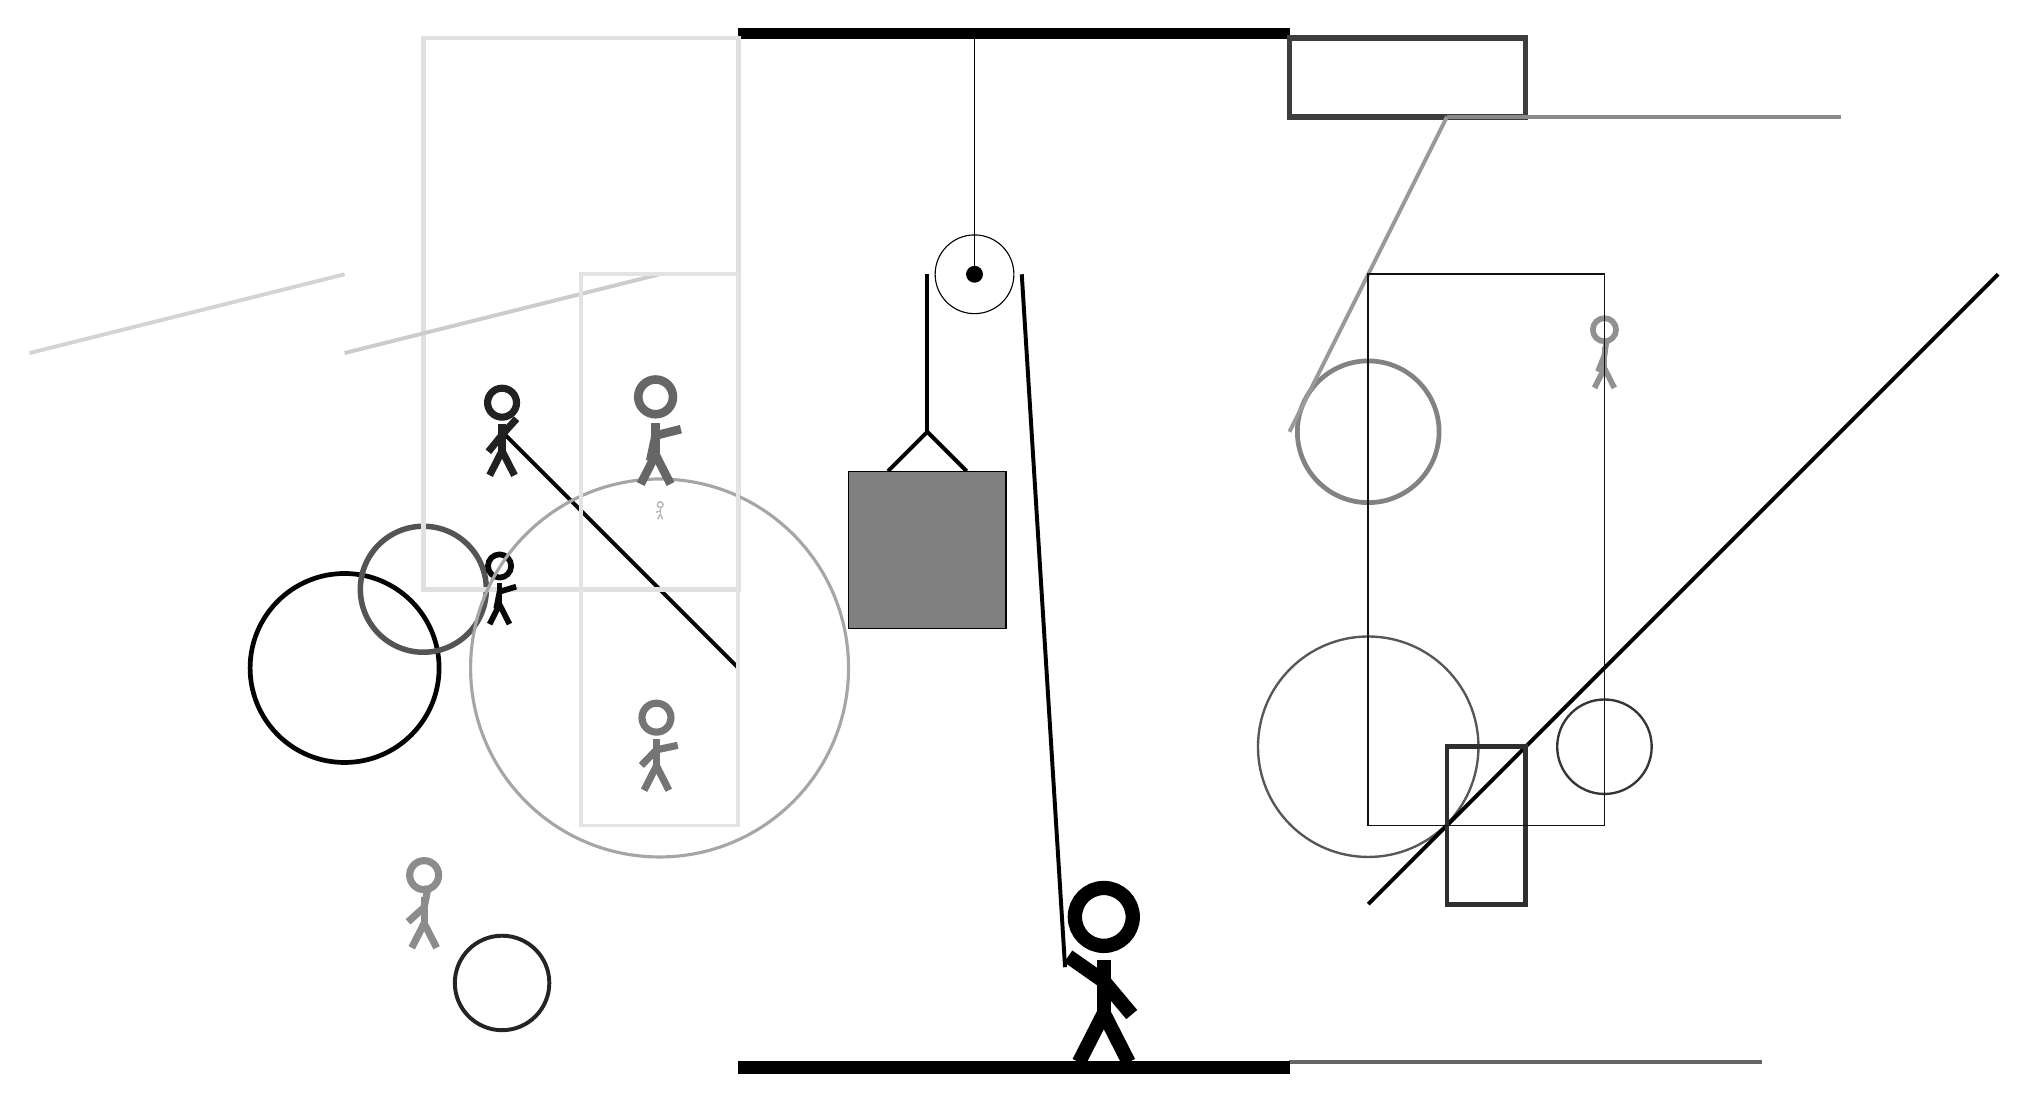
\begin{tikzpicture}
		%%%%% START %%%%%
		
		\draw[fill=black] (-2, 10) rectangle (5, 10.125);
		
		\draw (1, 7) circle (0.5);
		\draw[fill=black] (1, 7) circle (0.1);
		\draw (1, 10) -- (1, 7);
		
		\draw[line width=0.7mm, color=black!76] (5, 9) rectangle (8, 10);
		
		\draw [line width=0.6mm, color=black!99](-7, 2) circle (1.2);
		\draw[line width=0.5mm, color=black!98](-2, 2) -- (-5, 5);
		\draw[line width=0.5mm, color=black!17](-7, 7) -- (-11, 6);
		\draw [line width=0.7mm, color=black!67](-6, 3) circle (0.8);
		\draw [line width=0.6mm, color=black!49](6, 5) circle (0.9);
		\node[line width=0.4mm, color=black!43] at (9, 6) {\Strichmaxerl[4][68][82]};
		\draw [line width=0.3mm, color=black!66](6, 1) circle (1.4);
		\node[line width=0.7mm, color=black!45] at (-6, -1) {\Strichmaxerl[5][42][79]};
		\node[line width=0.5mm, color=black!54] at (-3, 1) {\Strichmaxerl[5][46][12]};
		\draw[line width=0.6mm, color=black!12] (-2, 10) rectangle (-6, 3);
		\draw[line width=0.5mm, color=black!40](5, 5) -- (7, 9);
		\draw[line width=0.5mm, color=black!20](-7, 6) -- (-3, 7);
		
		\draw[line width=0.5mm, color=black!100](6, -1) -- (14, 7);
		\draw[line width=0.3mm, color=black!63] (-2, 0) rectangle (-3, 0);
		\node[line width=0.7mm, color=black!28] at (-3, 4) {\Strichmaxerl[1][14][80]};
		
		\draw [line width=0.5mm, color=black!86](-5, -2) circle (0.6);
		\node[line width=0.2mm, color=black!97] at (-5, 3) {\Strichmaxerl[4][79][17]};
		\draw[line width=0.6mm, color=black!82] (7, 1) rectangle (8, -1);
		\draw [line width=0.4mm, color=black!35](-3, 2) circle (2.4);
		\draw[line width=0.5mm, color=black!60](5, -3) -- (11, -3);
		\draw [line width=0.3mm, color=black!79](9, 1) circle (0.6);
		\draw[line width=0.2mm, color=black!93] (6, 0) rectangle (9, 7);
		\draw[line width=0.5mm, color=black!46](7, 9) -- (12, 9);
		\node[line width=0.6mm, color=black!60] at (-3, 5) {\Strichmaxerl[6][78][14]};
		
		\draw[line width=0.5mm, color=black!11] (-4, 0) rectangle (-2, 7);
		\node[line width=0.7mm, color=black!87] at (-5, 5) {\Strichmaxerl[5][51][48]};
		
		\draw[line width=0.5mm] (-0.1, 4.5) -- (0.4, 5.0) -- (0.9, 4.5);
		\draw[fill=black!50] (-0.6, 4.5) rectangle (1.4, 2.5);
		
		\draw[line width=0.5mm] (0.4, 7) -- (0.4, 5.0);
		\centerarc[line width=0.5mm](1, 7)(0:180:0.6);
		\draw[line width=0.5mm](1.6, 7) -- (2.15, -1.8);
		
		\node at (2.6, -1.9) {\Strichmaxerl[10][-35][-50]};
		
		\draw[fill=black] (-2, -3) rectangle (5, -3.15);
		
		%%%%% END %%%%%
	\end{tikzpicture}
\end{document}